\documentclass[12pt]{article}
%Gummi|065|=)
\usepackage{amsmath, amsfonts, amssymb}
\usepackage[margin=0.5in]{geometry}
\usepackage{xcolor}
\usepackage{graphicx}

%\usepackage{pifont}
\usepackage{amsmath}



\newcommand{\off}[1]{}
\DeclareMathSizes{20}{30}{20}{18}

\newcommand{\two }{\sqrt[3]{2}}
\newcommand{\four}{\sqrt[3]{4}}
\newcommand{\red}{\begin{tikz}[scale=0.25]
\draw[fill=red, color=red] (0,0)--(1,0)--(1,1)--(0,1)--cycle;\end{tikz}}
\newcommand{\blue}{\begin{tikz}[scale=0.25]
\draw[fill=blue, color=blue] (0,0)--(1,0)--(1,1)--(0,1)--cycle;\end{tikz}}
\newcommand{\green}{\begin{tikz}[scale=0.25]
\draw[fill=green, color=green] (0,0)--(1,0)--(1,1)--(0,1)--cycle;\end{tikz}}

\newcommand{\sq}[3]{\draw[#3] (#1,#2)--(#1+1,#2)--(#1+1,#2+1)--(#1,#2+1)--cycle;}

\usepackage{tikz}
\usetikzlibrary{decorations.markings}

\newcommand{\susy}{{\bf Q}}
\newcommand{\RV}{{\text{R}_\text{V}}}

\title{Scratchwork: Theta Functions}
\date{}
\begin{document}

%\fontfamily{qag}\selectfont \fontsize{12.5}{15}\selectfont

\sffamily

\maketitle

\noindent William Duke's proof that the solutions to $n = a^2 + b^2 + c^2$ become equidistributed as $n \to \infty$ takes a quarter of a page:
\begin{itemize}
\item Goro Shimura shows there are many theta functions, each invariant under $\Gamma_0(4)$
$$ \theta(z;u) = \sum_{m \in \mathbb{Z}^3} u(m) \, e(z |m|^2) =
\sum_{n > 0} n^{\ell / 2}\, r_3(n) \left[ \frac{1}{r_3(n)} \sum_{\xi \in V_3(n)} u(\xi) \right] e ( n z)  $$
one for each spherical Harmonic $u \in L^2( S^2)$. Here $|m|^2 = m_1^2 + m_2^2 + m_3^2$ and $V_3(n) = \#\{ (a,b,c): a^2 + b^2 + c^2 = m \}$.
\item Henryk Iwaniec offers a bound for the Fourier coffients of cusp forms. 
$$ a_n \ll_{k, \epsilon} n^{k/2 - 2/7 + \epsilon} $$
These are tending to zero if we fix a tolerance  ($\epsilon$) and a ``weight" of modular form ($k$).
\item Combining Iwaniec and Shimura's result\footnote{and an estimate of Siegel, which I haven't even looked at, $r_3(n) \gg_\epsilon \sqrt{n^{1-\epsilon}} $.} we obtain an estimate for the sphere averages
$$  \frac{1}{r_3(n)} \sum_{\xi \in V_3(n)} u(\xi) \ll_{u,\epsilon} n^{-1/28 + \epsilon} $$
This bound depends on the spherical harmonic ($u$) and the tolerance ($\epsilon$).  And we need $n \not \equiv 7 \pmod 8$.  
\end{itemize}
So\dots what's good and bad about this style of argument.  It looks like a small tournament: \\ \\
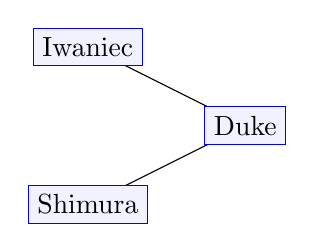
\begin{tikzpicture}



\draw (0,0)--(2,1);
\draw (0,2)--(2,1);

\node[rectangle, draw = blue, fill=blue!5] at (0,0) {Shimura};
\node[rectangle, draw = blue, fill=blue!5] at (0,2) {Iwaniec};
\node[rectangle, draw = blue, fill=blue!5] at (2,1) {Duke};

\end{tikzpicture}\hspace{2in}
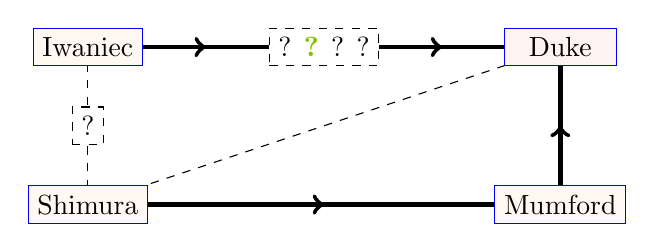
\begin{tikzpicture}


\draw[dashed] (0,0)--(6,2);
\draw[ultra thick] (0,2)--(3,2);
\draw[ultra thick] (3,2)--(6,2);
\draw[ultra thick] (0,0)--(6,0)--(6,2);
\draw[->, ultra thick](0,0)--(3,0);
\draw[->, ultra thick](0,2)--(1.5,2);
\draw[->, ultra thick](3,2)--(4.5,2);
\draw[->, ultra thick](6,0)--(6,1);
\draw[dashed] (0,0)--(0,2);

\node[rectangle, draw = blue, fill=orange!5] at (0,0) {Shimura};
\node[rectangle, draw = blue, fill=orange!5] at (0,2) {Iwaniec};
\node[rectangle, draw = blue, fill=red!5] at (6,2) {\;\;Duke\;\;};
\node[rectangle, draw = black, dashed, fill=white] at (3,2) {? {\color{green!50!orange}\textbf{?}} ? ?};
\node[rectangle, draw = blue, fill=orange!5] at (6,0) {Mumford};
\node[rectangle, fill=white, draw=black, dashed] at (0,1) {?};
\end{tikzpicture} \\ 
Here are some complaints I have about this proof:
\begin{itemize}
\item Duke uses theta functions  $\theta(z;u)$, while Iwaniec's bound works for \textit{any} cusp form.
\item Iwaniec expands an arbitrary (anonymous) $\Gamma_0(4)$ cusp form (or $\Gamma_0(N)$ for $N \equiv 0 (4)$) into Poincare series, which generalize Eisenstein series, which expand over the cusps of $SL(2, \mathbb{Z})/\Gamma_0(4)$.  Is there a more ``familiar" way of indexing this set? Perhaps I'd like to identify the cusps as a subset of the real axis $\mathbb{Q} \subseteq \mathbb{R} \simeq \{ x + 0i : x \in \mathbb{R}  \} \subseteq \mathbb{H} $  
\item The Fourier expansion of theta function $\theta(z;u)$ is just the q-series.  Iwaniec takes the Fourier expansion of Poincar\'{e} series from a textbook - the answer is a mix of Bessel functions and Kloosterman sums, which he estimates with much difficulty.
\item Do the sphere-averages lead naturally to Kloosterman sums?  Once he has written about the primes, we have basically used ``{strong approximation}" machinery, the kind of heavy machinery that Serre uses to guarantee even \textit{one} solution to $x^2 + y^2 + z^2 = n$.
\end{itemize}
Are there more down-to-earth ways to solve these problems?\footnote{I just refuse to believe this is best we can do.  We've learned this kind of problem has an inherent complexity about it, which has been explored in only the most abstract terms. There has to be an easier way to extract a discussion about individual cases that we care about.} Maybe not. Sadly, the ``advanced" approach and the ``elementary" approach look about the same.  The challenge is to state what we've contributed.\footnote{Going on vacation!  We can fly, drive, take the train, sail a boat, bicycle.  One more more of these may be appropriate.} \\ \\
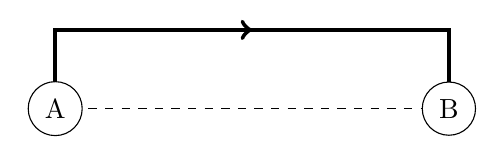
\begin{tikzpicture}
\draw[dashed] (0,0)--(5,0);
%\draw[->, ultra thick, dashed](0,0)--(2.5,0);
\draw[ultra thick] (0,0)--(0,1)--(5,1)--(5,0);
\draw[->, ultra thick] (0,1)--(2.5,1);

\node[circle, fill=white, draw=black] at (0,0) {A};
\node[circle, fill=white, draw=black] at (5,0) {B};
\end{tikzpicture} \\
E.g. The Waldspurger formula, is an equivalence between two objects that almost defy any description. So, I will have contributed an ``evaluation" of some kind of the Left and Right sides.

\vfill

\begin{thebibliography}{}

\item Anton Deitmar \textbf{Automorphic Forms} (Universitext \# ) Springer, 2013.
\item Françoise Dal'Bo  \textbf{Geodesic and Horocyclic Trajectories} Universitext, 2011.
\item Manfred Einsiedler, Thomas Ward. \textbf{Ergodic Theory (with a view towards Number Theory)} \\ GTM \#259, Springer 2011.
\item Yves Coudene  \textbf{
Ergodic Theory and Dynamical Systems} Universitext.  Springer, 2016.
\item Joel H. Shapiro \textbf{
A Fixed-Point Farrago} Universitext.  Springer, 2016.
\item \dots everything \dots
\item Akshay Venkatesh \textbf{Sparse equidistribution problems, period bounds, and subconvexity} \\ \texttt{arXiv:math/0506224} Annals of Mathematics, 172 (2010), 989-1094

\end{thebibliography}

\end{document}